\tikzset{>=latex} % for LaTeX arrow head
\colorlet{Ecol}{orange!90!black}
\colorlet{EcolFL}{orange!90!black}
\colorlet{veccol}{green!45!black}
\colorlet{Bcol}{violet!90}
\colorlet{Bcol1}{violet!80!blue!90}
\colorlet{Bcol2}{violet!80!red!90}
\colorlet{BFcol}{red!60!black}
\colorlet{veccol}{green!45!black}
\colorlet{Icol}{blue!70!black}
\tikzstyle{BField}=[->,thick,Bcol]
\tikzstyle{current}=[->,Icol,thick]
\tikzstyle{force}=[->,thick,BFcol]
\tikzstyle{vector}=[->,thick,veccol]
\colorlet{pluscol}{red!60!black}
\colorlet{minuscol}{blue!60!black}
\tikzstyle{charge+}=[very thin,draw=black,top color=red!50,bottom color=red!90!black,shading angle=20,circle,inner sep=0.3]
\tikzstyle{charge-}=[very thin,draw=black,top color=blue!50,bottom color=blue!80,shading angle=20,circle,inner sep=0.3]
\tikzstyle{metal}=[top color=black!15,bottom color=black!25,middle color=black!20,shading angle=10]
\tikzstyle{light metal}=[top color=black!10,bottom color=black!15,middle color=black!6,shading angle=10]
\tikzset{
  EFieldLine/.style={thick,EcolFL,decoration={markings,mark=at position #1 with {\arrow{latex}}},
                     postaction={decorate}},
  EFieldLine/.default=0.5,
  BFieldLine/.style={thick,Bcol,decoration={markings,mark=at position #1 with {\arrow{latex}}},
                                 postaction={decorate}},
  BFieldLine/.default=0.5,
  pics/Bin/.style={
    code={
      \def\R{0.12}
      \draw[pic actions,line width=0.6,#1,fill=white] % ,thick
        (0,0) circle (\R) (-135:.75*\R) -- (45:.75*\R) (-45:.75*\R) -- (135:.75*\R);
  }},
  pics/Bout/.style={
    code={
      \def\R{0.12}
      \draw[pic actions,line width=0.6,#1,fill=white] (0,0) circle (\R);
      \fill[pic actions,#1] (0,0) circle (0.3*\R);
  }},
  pics/Bin/.default=Bcol,
  pics/Bout/.default=Bcol,
  pics/magnet/.style={ %args={#1}
    code={
      \def\h{0.9}
      \coordinate (-N) at (0,\h);
      \coordinate (-S) at (0,-\h);
      \draw[pic actions,thick,top color=red!60,bottom color=red!90,shading angle=20]
        (-0.8*\h/2,0) rectangle ++(0.8*\h,\h);
      \draw[pic actions,thick,top color=blue!60,bottom color=blue!90,shading angle=20]
        (-0.8*\h/2,0) rectangle ++(0.8*\h,-\h);
      \node[pic actions] at (0, \h/2) {\textbf{N}};
      \node[pic actions] at (0,-\h/2) {\textbf{S}};
  }},
}
\tikzstyle{measure}=[<->,fill=white,midway,outer sep=0]
\contourlength{1.5pt}

% FLUX-CHANGING LOOP


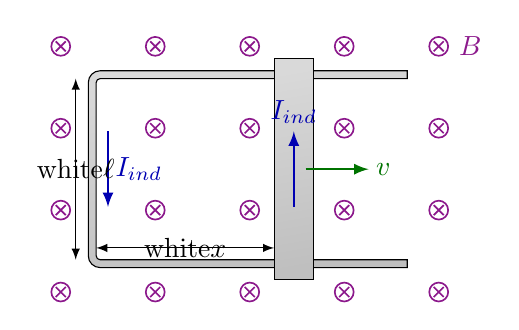
\begin{tikzpicture}
  \def\NBx{5}
  \def\NBy{4}
  \def\L{4.0}
  \def\W{2.4}
  \def\d{4.0}
  \def\t{0.1}
  \def\s{0.64}
  
  % MAGNETIC FIELDLINES
  \foreach \i [evaluate={\y=-0.15*\W+(\i-1)*1.3*\W/(\NBy-1)}] in {1,...,\NBy}{
    \foreach \j [evaluate={\x=-0.1*\L+(\j-1)*1.2*\L/(\NBx-1)}] in {1,...,\NBx}{
      \pic[scale=1] at (\x,\y) {Bin};
    }
  }
  \node[Bcol] at (1.2*\L,1.15*\W) {$\vb{B}$};
  
  % WIRE
  \draw[metal] (\L,\t/2) -- (\t,\t/2) arc (-90:-180:\t/2) -- (\t/2,\W-\t) arc (180:90:\t/2)
                         -- (\L,\W-\t/2) -- (\L,\W+\t/2) -- (\t,\W+\t/2) arc (90:180:1.5*\t)
                         -- (-\t/2,\t) arc (-180:-90:1.5*\t) -- (\L,-\t/2) -- cycle;
  \draw[metal] (\s*\L-2.5*\t,-2*\t) rectangle++ (5*\t,\W+4*\t);
  \draw[vector] (\s*\L+1.5*\t,\W/2) --++ (0.2*\L,0) node[right=-1] {$\vb{v}$};
  \draw[current] (\s*\L,0.3*\W) --++ (0,0.4*\W) node[above=-1] {$I_\text{ind}$};
  \draw[current] (2*\t,0.7*\W) --++ (0,-0.4*\W) node[midway,right=-1] {$I_\text{ind}$};
  \draw[<->] (\t/2,2*\t) -- (\s*\L-2.5*\t,2*\t) node[midway] {\contour{white}{$x$}};
  \draw[<->] (-2.1*\t,\t/2) -- (-2.1*\t,\W-\t/2) node[midway] {\contour{white}{$\ell$}};
  
\end{tikzpicture}
